\subsection{Platform Initialization \gls{pi} Boot Sequence}
PI compliant system firmware must support the six phases: security (\gls{sec}), pre-efi initialization (\gls{pei}), driver execution environment (\gls{dxe}), boot device selection (\gls{bds}), run time (RT) services and After Life (transition from the OS back to the firmware) of system. Refer to Figure \ref{fig:design-pi-boot-phases} below.

\begin{figure}[h]
	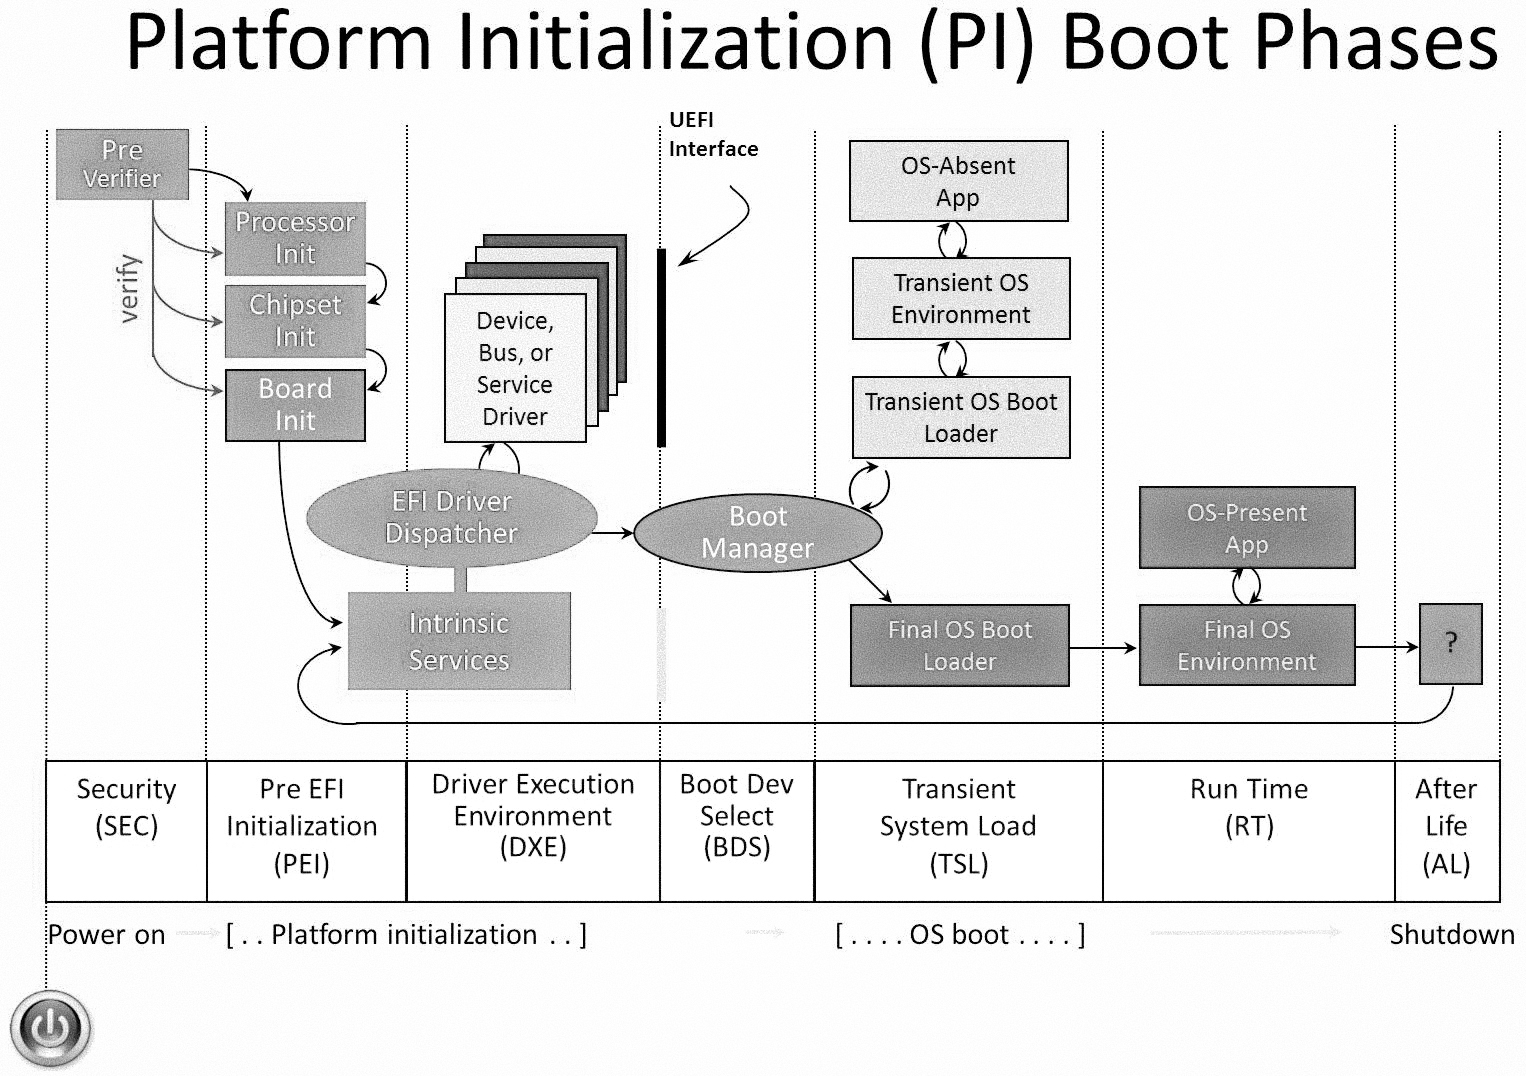
\includegraphics[width=\linewidth]{PI_Boot_Phases}
	\caption{\gls{pi} Boot Phases}\label{fig:design-pi-boot-phases}
\end{figure}

\subsubsection{Security (\gls{sec})}
The Security (SEC) phase is the first phase in the PI Architecture and is responsible for the following:
\begin{itemize}
	\item Handling all platform restart events
	\item Creating a temporary memory store
	\item Serving as the root of trust in the system
	\item Passing handoff information to the PEI Foundation
\end{itemize}
The security section may contain modules with code written in assembly. Therefore, some EDK II module development environment (MDE) modules may contain assembly code. Where this occurs, both Windows and GCC versions of assembly code are provided in different files

\subsubsection{Pre-EFI Initialization (\gls{pei})}
The Pre-EFI Initialization (PEI) phase described in the PI Architecture specifications is invoked quite early in the boot flow. Specifically, after some preliminary processing in the Security (SEC) phase, any machine restart event will invoke the PEI phase.
The PEI phase initially operates with the platform in a nascent state, leveraging only on-processor resources, such as the processor cache as a call stack, to dispatch Pre-EFI Initialization Modules (PEIMs). These PEIMs are responsible for the following:
\begin{itemize}
	\item Initializing some permanent memory complement
	\item Describing the memory in Hand-Off Blocks (HOBs)
	\item Describing the firmware volume locations in HOBs
	\item Passing control into the Driver Execution Environment (DXE) phase
\end{itemize}

\subsubsection{Drive Execution Environment (\gls{dxe})}
Prior to the DXE phase, the Pre-EFI Initialization (PEI) phase is responsible for initializing permanent memory in the platform so that the DXE phase can be loaded and executed. The state of the system at the end of the PEI phase is passed to the DXE phase through a list of position independent data structures called Hand-Off Blocks (HOBs). HOBs are described in detail in the Platform Initialization Specification.
There are several components in the DXE phase:
\begin{itemize}
	\item DXE Foundation
	\item DXE Dispatcher
	\item A set of DXE Drivers
\end{itemize}

\subsubsection{Boot Device Selection (\gls{bds})}
The Boot Device Selection (BDS) phase is implemented as part of the BDS Architectural Protocol. The DXE Foundation will hand control to the BDS Architectural Protocol after all of the DXE drivers whose dependencies have been satisfied have been loaded and executed by the DXE Dispatcher. The BDS phase is responsible for the following:
\begin{itemize}
	\item Initializing console devices
	\item Loading device drivers
	\item Attempting to load and execute boot selections
\end{itemize}

\subsubsection{Transient System Load (TSL) and Runtime (RT)}
The Transient System Load (TSL) is primarily the OS vendor provided boot loader. Both the TSL and the Runtime Services (RT) phases may allow access to persistent content, via UEFI drivers and UEFI applications. Drivers in this category include PCI Option ROMs.

\subsubsection{After Life (AL)}
The After Life (AL) phase consists of persistent UEFI drivers used for storing the state of the system during the OS orderly shutdown, sleep, hibernate or restart processes.
